\documentclass[a4paper,12pt]{report}

\usepackage[utf8]{inputenc}
\usepackage{graphicx}
\usepackage{amsmath}
\usepackage{amssymb}
\usepackage{hyperref}
\usepackage{geometry}
\usepackage{titling}
\usepackage{graphicx}
\usepackage{hyperref}
\usepackage{acro}
\usepackage{csquotes}
\usepackage{caption}
\usepackage{svg}
\usepackage{float}
\usepackage{nomencl}

\geometry{margin=1in}


\setsvg{inkscape={"C:/Program Files/Inkscape/inkscape"}}

\DeclareAcronym{gsoc}{
	short=GSoC,
	long=Google Summer of Code
}

\DeclareAcronym{grc}{
	short=GRC,
	long=GNU Radio Companion
}

\DeclareAcronym{ula}{
	short=ULA,
	long=Uniform Linear Array
}

\DeclareAcronym{oot}{
	short=OOT,
	long=Out-Of-Tree
}

\DeclareAcronym{doa}{
	short=DoA,
	long=Direction-of-Arrival
}

\DeclareAcronym{ura}{
	short=URA,
	long=Uniform Rectangular Array
}

\DeclareAcronym{uca}{
	short=UCA,
	long=Uniform Circular Array
}

\DeclareAcronym{gr}{
	short=GR,
	long=GNU Radio
}

\DeclareAcronym{mvdr}{
	short=MVDR,
	long=Minimum Variance Distortionless Response
}

\DeclareAcronym{lcmv}{
	short=LCMV,
	long=Linearly Constrained Minimum Variance
}

\DeclareAcronym{music}{
	short=MUSIC,
	long=MUltiple Signal Classification
}

\DeclareAcronym{gui}{
	short=GUI,
	long=Graphical User Interface
}

\DeclareAcronym{hpbw}{
	short=HPBW,
	long=Half-Power Beamwidth
}

\DeclareAcronym{nnbw}{
	short=NNBW,
	long=Null-to-Null Beamwidth
}

\DeclareAcronym{sll}{
	short=sll,
	long=Side-Lobe Level
}

\DeclareAcronym{ui}{
	short=UI,
	long=User Interface
}

\begin{document}
	
	\begin{titlepage}
		\centering
		\vspace*{1cm}
		
		\Huge \textbf{Array Processing ToolBox}
		
		\vspace{0.5cm}
		\Large gr-array
		
		\vspace{1.5cm}
		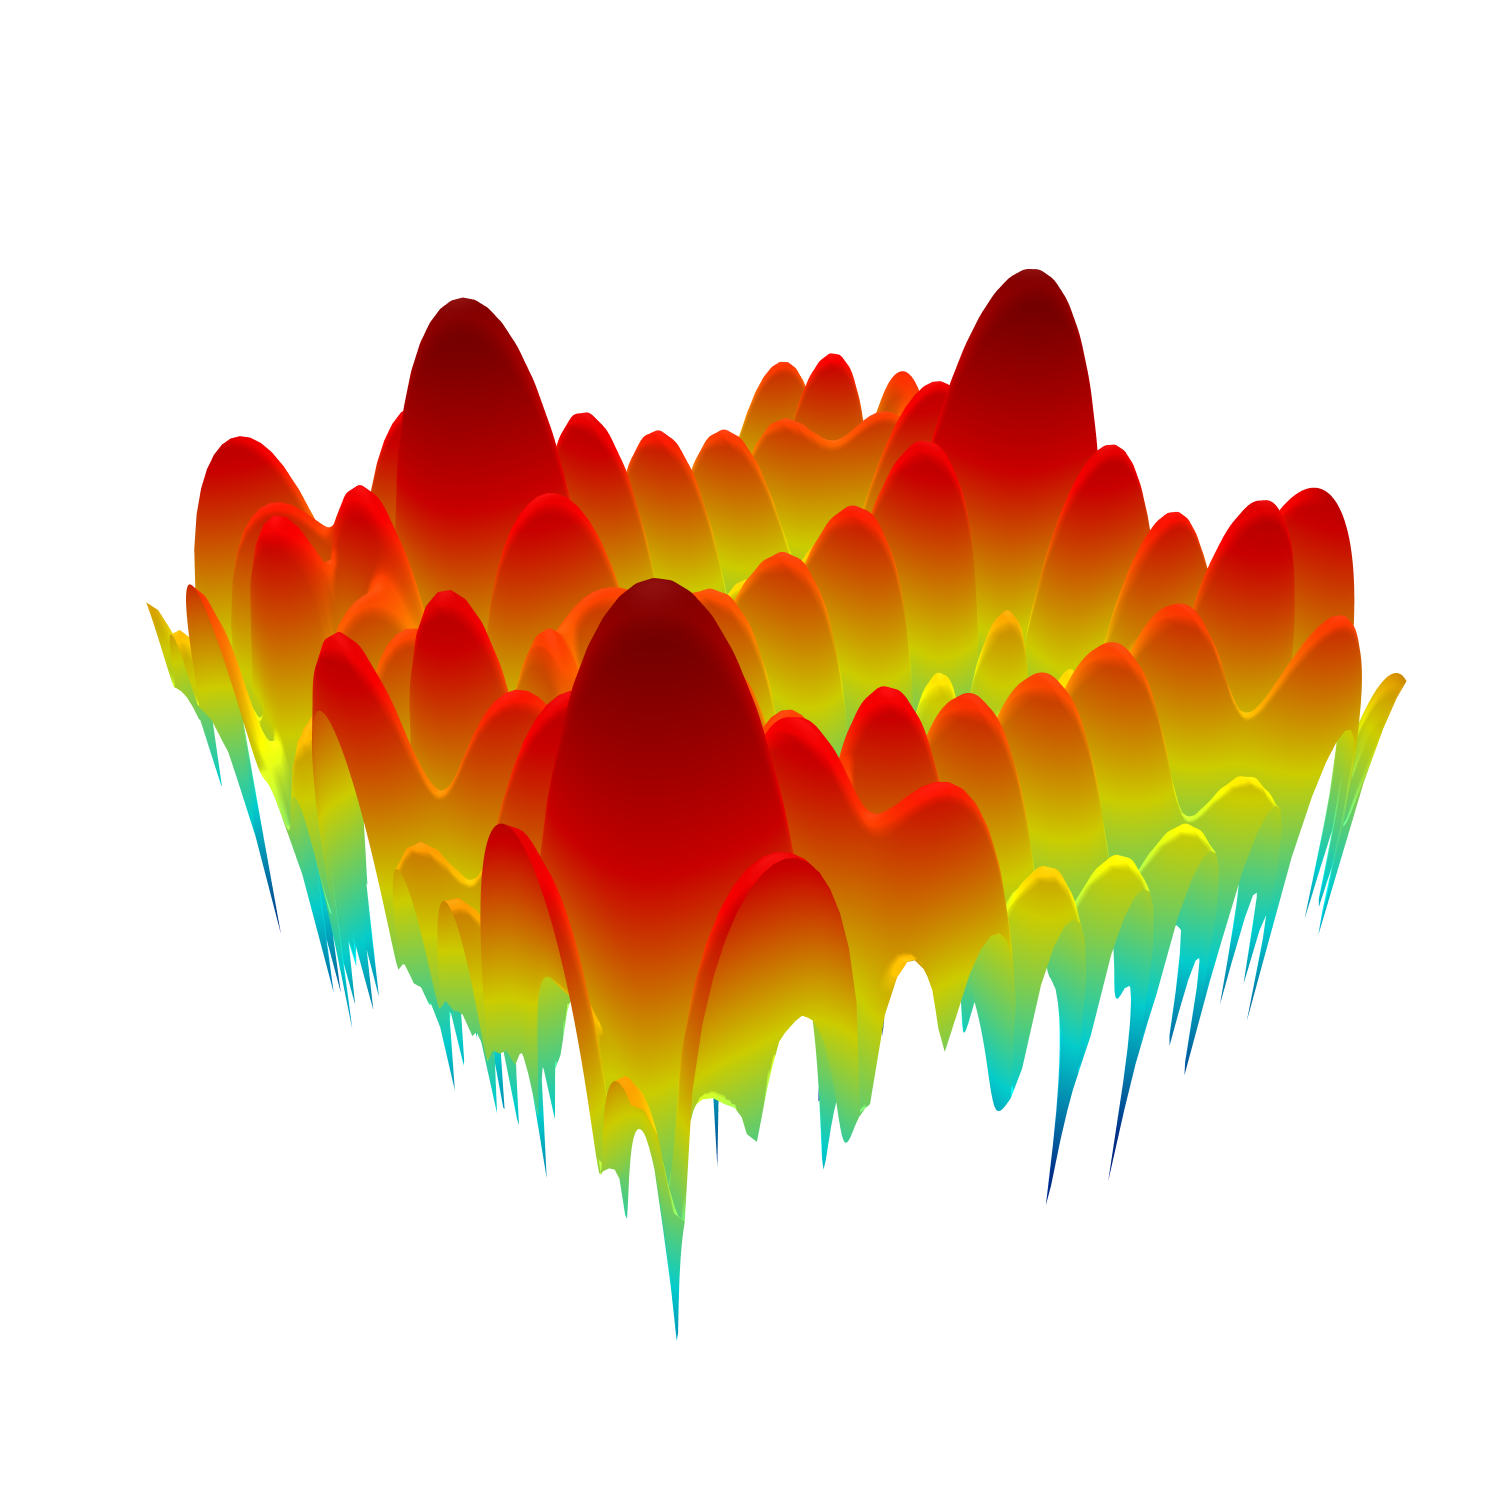
\includegraphics[scale=0.3]{images//title_doa}
		
		\vspace{1.5cm}
		\textbf{Author:} Rahul Rajeev Pillai
		
		\vfill
		
		\textbf{Date:} \today
				
	\end{titlepage}

	\setcounter{page}{1}
	\pagenumbering{roman}
	
	\chapter*{Abstract}
\addcontentsline{toc}{chapter}{Abstract}

This is a proposal for a project that seeks to create a tool for designing and analyzing sensor arrays in GNU Radio. The tool will feature a user-friendly GUI to configure array parameters, visualize patterns, analyze performance metrics, and experiment with various built-in array processing algorithms. It will also generate \acf{gr} flow graphs based on the user-defined parameters, enabling seamless transition from design to real-time testing withing the GNU Radio. This project strives to make advanced array processing more accessible, fostering exploration and innovation without relying on proprietary software.

	
	\clearpage
	\tableofcontents
	\addcontentsline{toc}{chapter}{Table of Contents}
	
	\clearpage
	\listoffigures
	\addcontentsline{toc}{chapter}{List of Figures}
	
	\clearpage
	\listoftables
	\addcontentsline{toc}{chapter}{List of Tables}
	
	\clearpage
	\printacronyms[sort=true, name=List of Abbreviations]
	\addcontentsline{toc}{chapter}{List of Abbreviations}
	
	\clearpage
	\setcounter{page}{1}
	\pagenumbering{arabic}
	
	\chapter{Introduction} \label{ch: introduction}

\section{Project Overview}

This project aims to develop an open-source, interactive tool for designing and analyzing sensor arrays within \acf{gr}, it is inspired by MATLAB’s \href{https://in.mathworks.com/products/phased-array.html}{Phased Array System Toolbox} (more specifically: \href{https://in.mathworks.com/help/phased/ref/sensorarrayanalyzer-app.html}{Sensor Array Analyzer}). This \acs{gui}-based tool should allow users to configure various array parameters, visualize the array-factor in different plots, and play around with popular Beamforming and \acf{doa} estimation algorithms.

Once the design is complete, the tool should generate a compatible \ac{gr} flow graph, configured with the chosen array settings. This functionality bridges the gap between array design and real-time testing, empowering researchers and engineers to iterate and test their designs seamlessly in \ac{gr}.

By creating this tool, the project seeks to provide the open-source community with a powerful, accessible alternative to proprietary software, lowering the barrier to entry for advanced array processing research and development.
	
\section{Motivation}

When I first started as an intern, I was tasked with developing adaptive array algorithms. At the time, my understanding of signal processing was very limited, and working with multi-dimensional signal processing algorithms was really a daunting task. The first major hurdle was grasping the mathematical foundations and intuition behind the algorithms. After extensive effort, I was able to develop a good understanding of most concepts.

The next challenge was implementation and verification. While searching for simulation tools, I found that MATLAB was the primary option, but being paid-license based, I was unable to use it. This left me with no choice but to develop everything from scratch. At that time, my programming experience was limited, making the process even more difficult. I looked online for array processing algorithm implementations to get a sense of how they were implemented. Although there were only a handful of resources available, I managed to find a couple of GitHub repositories and \href{https://pysdr.org/}{PySDR}, which proved to be invaluable. They helped me with signal generation, algorithm implementation, pattern visualization, and even understanding the underlying theory. However, they primarily focused on \acf{ula}, making it quite tricky to do the same for planar arrays. Through extensive study of textbooks and careful adaptation of available resources, I was eventually able to extend the simulation to planar array.

While I gained a lot from developing everything from scratch, it was also time-intensive and prone to errors. Developing the core algorithm is one aspect, but implementing signal generation, visualization tools and all the other supporting tools, just adds significant overhead. This project aims to simplify these aspects, allowing researchers and engineers to focus on algorithm development rather than spending excessive time on auxiliary tasks.

\section{Objective} \label{sec: objective}

\begin{itemize}
	\item \textbf{OBJ-1}: To develop an interactive graphical tool that enables a user to configure various parameters of a sensor array and visualize the array factor using different plotting methods.
	\item \textbf{OBJ-2}: The graphical tool should be able to simulate different array processing algorithms for various user-defined array configurations and parameters and provide immediate results.
	\item \textbf{OBJ-3}: The tool should include a mechanism to convert the user-defined configurations into a valid \acl{gr} compatible flow graph.
	
\end{itemize}

\section{Milestones} \label{sec: milestones}

\begin{itemize}
	\item \textbf{MS-1}: Planning
	\begin{itemize}
		\item Connect with mentors and the community.
		\item Iron out details of the project.
		\item Setup work environment.
	\end{itemize}
	\item \textbf{MS-2}: \acf{gui}.
	\begin{itemize}
		\item Set up the GUI framework.
		\item Implement user-friendly input controls.
		\item Ensure smooth navigation and parameter configuration.
	\end{itemize}
	\item \textbf{MS-3}: Signal Processing Library.
	\begin{itemize}
		\item Implement a function for steering vector generation based on different parameters for a wide range of array configurations.
		\item Develop a library of array processing algorithms in Beamforming and \ac{doa} estimation.
	\end{itemize}
	\item \textbf{MS-4}: Development of \ac{oot} modules and flow graph generation.
	\begin{itemize}
		\item Create a set of customizable \ac{grc} blocks designed to meet diverse user settings.
		\item Implement a functionality within the application window that allows the user to convert their settings to a flow graph in \acl{gr}.
	\end{itemize}
		\item \textbf{MS-5}: Integration.
	\begin{itemize}
		\item Develop a library for generating various types of plots.
		\item Integrate the signal processing library, plotting library, \ac{gui} and the flowgraph generator with the application window.
		\item Enable the window to be launched directly from within \ac{grc}.
	\end{itemize}
\end{itemize}

\begin{center}
	\captionof{table}{Objective - Milestone mapping.}
	\begin{tabular}{|c|c|c|c|c|c|c|}
		\hline
		& MS-1 & MS-2 & MS-3 & MS-4 & MS-5 \\ \hline
		OBJ-1 & 1    & 1    &  1    &     &   1         \\ \hline
		OBJ-2 & 1    &      &  1    &     &   1         \\ \hline
		OBJ-3 & 1    &      &       & 1   &   1    \\ \hline
	\end{tabular}
\end{center}

\section{Document Structure}

The remainder of this proposal is structured as follows:

\begin{itemize}
	
	\item \textbf{Chapter \ref{ch: project-systems}}: Project Systems \\
	\indent Describes the high-level system architecture. It details how the project is divided into multiple systems  components such as the application window, signal processing library, and \ac{oot} module and are structured to work together.
	
	\item \textbf{Chapter \ref{ch: application-window}}: Application Window \\
	\indent Explains the graphical interface for the project. It gives an idea on how the \ac{ui} will look like and explains the different panes of the window. It also goes into the different types of plotting methods that are available and how it is connected to the signal processing library.
	
	\item \textbf{Chapter \ref{ch: signal-processing-library}}: Signal Processing Library \\
	\indent Details the development of core signal processing functions including steering vector generation, beamforming techniques, and DoA estimation algorithms.
	
	\item \textbf{Chapter \ref{ch: oot-modules}}: \acf{oot} Modules \\
	\indent Describes the implementation of custom \acl{gr} \ac{oot} blocks that expose array processing functionalities in the \ac{grc} environment. This chapter gives a brief introduction to the \ac{oot} modules that will be developed for seamless transition between design and testing in \ac{gr}.
	
\end{itemize}




	\chapter{Project Systems} \label{ch: project-systems}

This entire project can be divided into 3 main components.

\begin{itemize}
	\item Application Window
	\item Signal Processing Library
	\item \ac{oot} modules
\end{itemize}

\section{Application Window}

\begin{figure}[h]
	\centering
	\includesvg[scale=1]{images//app-window} % Rotates 90 degrees
	\caption{Application Window and its sub-systems.}
\end{figure}

The application window acts as the main interface for the user, bringing together array configuration, visualization, simulation, and flowgraph generation all in a single environment.

It will feature an intuitive \ac{gui} with controls like sliders, dropdowns, and text fields to allow users to easily set array parameters, visualize beam patterns etc. The window will also offer simulation capabilities for array processing algorithms and support automatic generation of flow graphs from user-defined settings that can be used in \acl{gr}.

To streamline the workflow, the application window can be launched directly from within \ac{grc}, ensuring smooth integration with the existing GNU Radio framework.

\section{Signal Processing Library}

\begin{figure}[h]
	\centering
	\includesvg[scale=1]{images//sig-processing-lib} % Rotates 90 degrees
	\caption{Signal Processing Library and its sub-systems.}
\end{figure}


The signal processing library forms the core component of the project, providing the computational backbone for array analysis and algorithm simulation.

The library will include functions for steering vector generation, supporting a variety of array geometries and parameter configurations. This ensures flexibility and adaptability across different sensor array setups. Additionally, it will have in-built functions of various Beamforming and \ac{doa} estimation, allowing users to evaluate and compare different techniques within the same framework.

To support meaningful analysis, the library will also provide tools to measure performance metrics of both the arrays and the implemented algorithms. These tools will be tightly integrated with the GUI and plotting modules, enabling quick simulation and visualization.

\section{\ac{oot} Modules}

\begin{figure} [h]
	\centering
	\includesvg[scale=1]{images//oot-modules} % Rotates 90 degrees
	\caption{OOT Modules.}
\end{figure}

As part of the system’s integration with \acl{gr}, a set of custom \ac{oot} modules will be developed to extend the platform’s native functionality and provide a seamless interface between the graphical tool (application window) and \acf{grc}. These \ac{oot} modules are designed to support user-defined array configurations and processing algorithms by using them as reusable blocks within the GRC environment.

Each block will encapsulate a specific array processing function, such as steering vector generation, beamforming, or direction-of-arrival (DoA) estimation, allowing users to incorporate these capabilities directly into their GNU Radio flowgraphs. The blocks will be implemented in C++ or Python, with proper XML code to ensure compatibility with the GRC graphical interface.

This modular design enables users to prototype and validate their array processing pipelines quickly, while maintaining the flexibility to modify and expand the processing chain as needed.

\section{System Integration}

The integration phase brings together all the major components of the project into a functional system. At the heart of this integration lies the seamless interaction between the application window, signal processing library, and the custom \ac{oot} modules from \ac{gr}.

\begin{figure}[H]
	\centering
	\includesvg[angle=90, scale=0.7]{images//project-systems} % Rotates 90 degrees
	\caption{System block diagram.}
\end{figure}

The application window serves as the primary user interface, enabling users to intuitively configure sensor array parameters, select array processing algorithms, and visualize the resulting beam patterns or estimation outputs. It acts as the front end through which all system functionalities are accessed.

Behind the scenes, the signal processing library performs the core computations. It houses essential algorithms for steering vector generation, Beamforming, and \ac{doa} estimation. The library is a separate entity common to the application window and the \ac{oot} modules and it is accessed through function calls.

To support real-world deployment and SDR experimentation, the system includes a set of custom OOT modules for \ac{gr}. The application window can generate \ac{gr}-compatible flow graphs based on the user's settings, enabling a smooth transition from design and simulation to real-world implementation in \ac{gr}.

Together, these components form a tightly integrated toolchain, from configuration and simulation to real-time execution and bridging the gap between intuitive design and SDR-based prototyping.
	\chapter{Application Window} \label{ch: application-window}

\begin{figure}[H]
	\centering
	\includesvg[scale=1]{images//app_window}
	\caption{Application Window.}
\end{figure}


The application window is the main container that holds all interface elements and the backend. It provides users with a cohesive environment to configure, run, and analyze the array with various parameters.

\section{\acf{gui}}

\begin{figure}[H]
	\centering
	\includesvg[scale=1]{images//window}
	\caption{Foundational \ac{gui} idea for the application window.}
\end{figure}

The \ac{gui} will consists of primarily two panes. Pane-1 will be for the user to input their configurations and settings. And Pane-2 will be for the visualizing the desired plot based on the user-defined settings. Typical parameters available will be,

\begin{itemize}
	\item Frequency
	\item inter-element spacing
	\item number elements
	\item array configurations
	\item angle-of arrival
\end{itemize}

\section{Signal Processing Backend}

This serves as the core engine that connects the user interface with the signal processing library. It receives configuration parameters from the GUI and uses them to initialize or update the processing chain. This backend handles tasks like generating steering vectors, applying beamforming algorithms, and performing DoA estimation using synthetic data. It communicates with the processing library and returns the computed results, which then can be plotted using the plotting library. This architecture ensures a modular responsive, and extensible system.

\section{Flow Graph Generator}

The Flow Graph Generator is a key component that automatically builds and configures a signal processing flow based on user input in \acl{gr}. Its main purpose is to translate high-level user-defined parameters into a structured and executable \ac{gr} flowgraph. This generator acts as a bridge between user-friendly GUI controls and the underlying processing blocks, ensuring that the right sequence of blocks is instantiated and connected in the \acf{grc}.

\section{Plotting library}

The Plotting Library is responsible for rendering all visual outputs in the application. It receives numerical data—like spatial spectra, array responses, or estimated angles—from the signal processing backend and generates clear, interactive plots in the Visualization Window (Pane-2). It includes different plotting methods like,

\begin{itemize}
	\item Contour plot
	\item Polar plot
	\item Cartesian plot
\end{itemize}

\clearpage
\begin{figure}[H]
	\centering
	\hspace*{-1.8cm}
	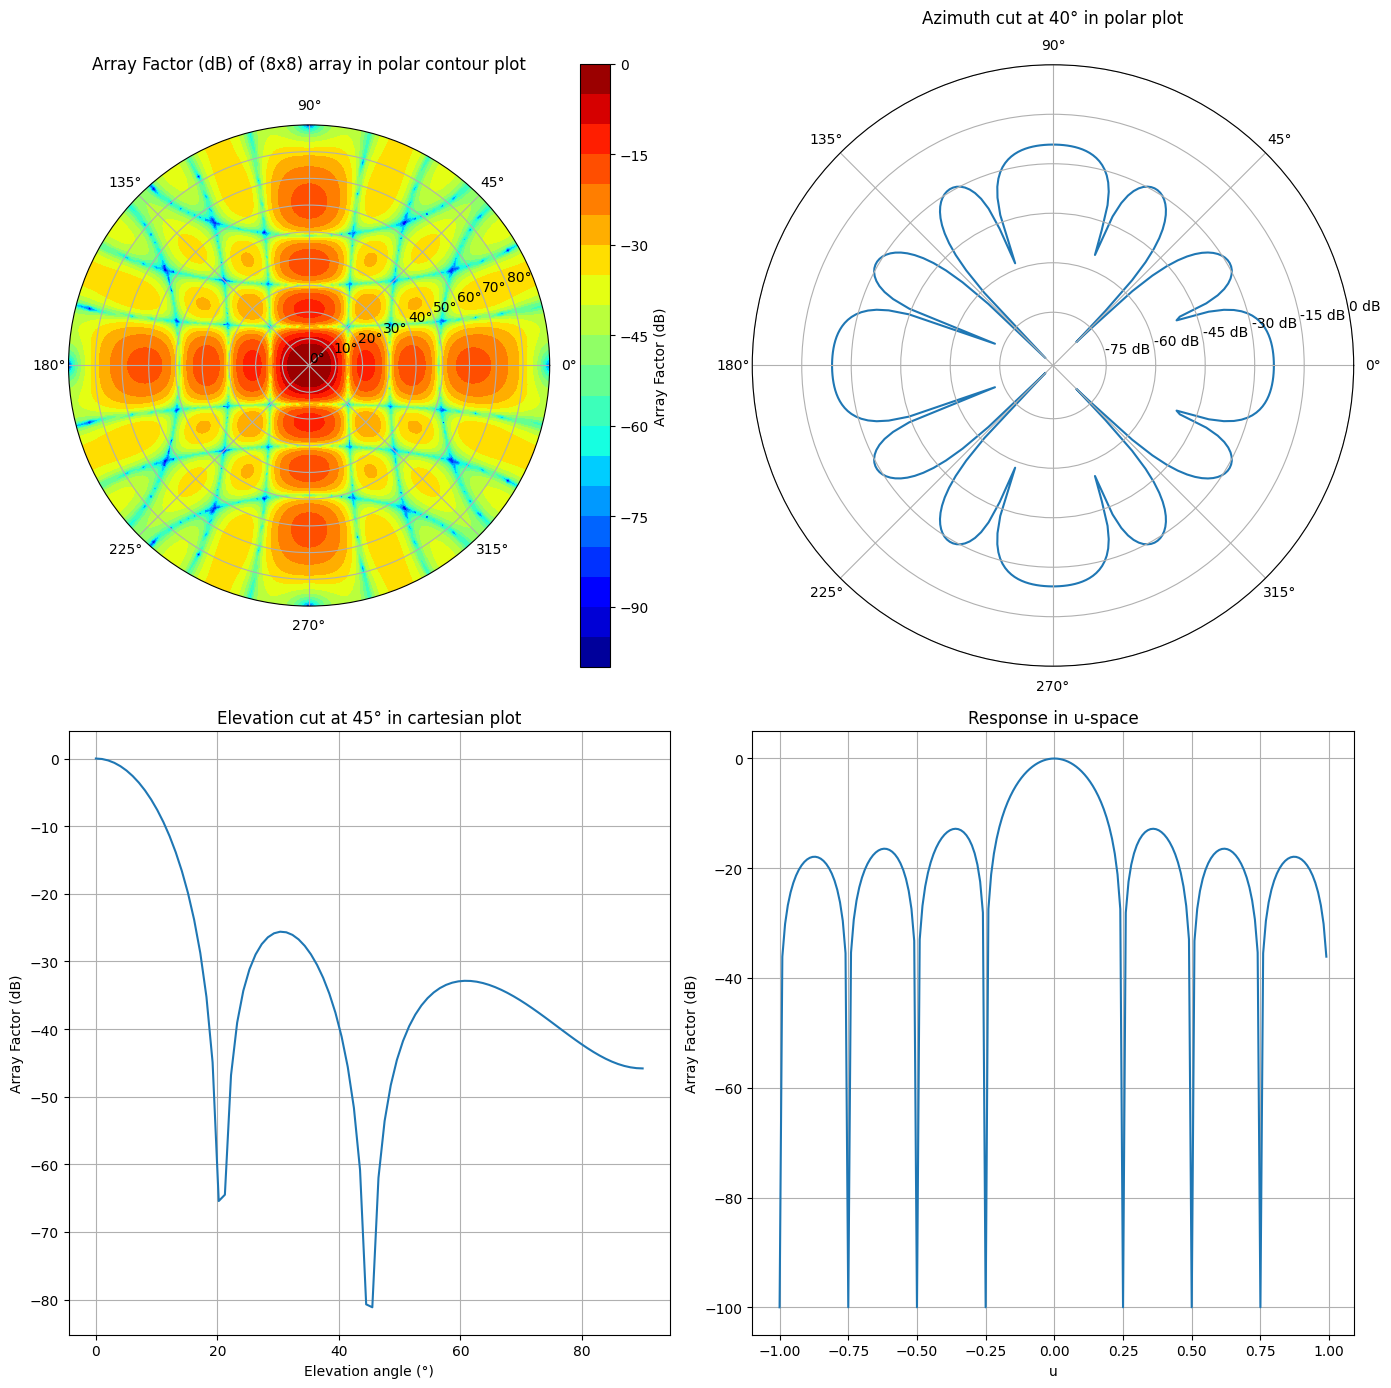
\includegraphics[scale=0.56]{images//plots}
	\caption{Different pattern visualization of an 8$\times$8 array.}
\end{figure}
	\chapter{Signal Processing Library} \label{ch: signal-processing-library}

\section{Array}

\begin{center}
	\renewcommand{\arraystretch}{1.5}
	\captionof{table}{Array configuration and its steering vector calculation.}
	\begin{tabular}{|c|c|}
		\hline
		Array & Steering Vector  \\ \hline
		\acl{ula}   & $\text{v}(\theta) = e^{-\text{j}2\pi \frac{\text{d}}{\lambda} n\sin(\theta)}$          \\ \hline
		\acl{ura}   & $\text{v}(\theta, \phi) = e^{-\text{j}2\pi \frac{1}{\lambda}( n\text{d}_x\sin(\theta)\cos(\phi) + m\text{d}_y\sin(\theta)\sin(\phi))}$                 \\ \hline
	\end{tabular}
\end{center}


where,
\begin{itemize}
	\item d - inter-element spacing in m.
	\item $\lambda$ - wavelength of the signal.
	\item $\theta$ - elevation angle in rad.
	\item $\phi$ - azimuth angle in rad.
	\item $\text{d}_x$ - inter-element spacing in x-axis (array normal is z-axis).
	\item $\text{d}_y$ - inter-element spacing in y-axis (array normal is z-axis).
	\item $n$ - index of the element in x-axis.
	\item $m$ - index of the element in y-axis.
	\item $\text{v}(\theta)$, $\text{v}(\theta, \phi)$ - steering vectors for \ac{ula} and \ac{ura} respectively.
 \end{itemize}

\section{Beamforming algorithm}

\begin{center}
	\renewcommand{\arraystretch}{1.5}
	\captionof{table}{Beamforming algorithm and its weights computation.}
	\begin{tabular}{|c|c|}
		\hline
		Algorithm & Weight computation  \\ \hline
		\acl{mvdr}   & $\text{w} = \frac{\text{R}^{-1} \text{v}}{\text{v}^{\text{H}} \text{R}^{-1} \text{v}}$          \\ \hline
		\acl{lcmv}   & $\text{w} = \frac{\text{R}^{-1} \text{C}}{\text{C}^{\text{H}} \text{R}^{-1} \text{C}} \delta$                 \\ \hline
	\end{tabular}
\end{center}

where, 

\begin{itemize}
	\item w - is the weight vector of the algorithm.
	\item $\text{R}^{-1}$ - inverse covariance matrix.
	\item v - steering vector (either from \ac{ula} or \ac{ura})
	\item C - constraint matrix.
	$$ \text{C} = \begin{bmatrix}
		\text{v}_0, \text{v}_1, \hdots \text{v}_i
	\end{bmatrix}$$ 
	v\textsubscript{$i$} refers to steering vector based on different directions. C contains all possible steering vector that are to be considered.
	\item $\delta$ - desired response matrix
	$$ \delta = \begin{bmatrix}
		1, 1, 0, \hdots 1
	\end{bmatrix} $$
	contains the desired response corresponding to the steering vector. 1 means beam and 0 means null.
\end{itemize}

\section{\ac{doa} Esimation algorihtm}

\begin{center}
	\renewcommand{\arraystretch}{1.5}
	\captionof{table}{\ac{doa} algorithm and its spectrum computation.}
	\begin{tabular}{|c|c|}
		\hline
		Algorithm & Spectrum computation  \\ \hline
		Beamscan   & $\text{P}(\theta, \phi) = \text{v}^\text{H} \text{R} \text{v}$          \\ \hline
		\acl{mvdr}   & $\text{P}(\theta, \phi) = \frac{1}{\text{v}^{\text{H}} \text{R}^{-1} \text{v}} $              \\ \hline
	\end{tabular}
\end{center}

where,

\begin{itemize}
	\item $\text{P}(\theta, \phi)$ - refers to the power spectrum.
	 
\end{itemize}

	\chapter{\acf{oot} Modules} \label{ch: oot-modules}

\begin{itemize}
	\item \textit{Array Response}: A \acs{gr} block that receives multiple input signals and outputs $N$ phase-shifted versions of the superimposed signal based on the steering vector.
	\item \textit{Steering Vector}: A \ac{gr} block that can be configured to generate phase delays based on the array configurations.
	\item \textit{Beamforming}: A \ac{gr} block that takes in $N$ phase-shifted signals and apply popular beamforming algorithms.
	\item \textit{\acs{doa} Estimation}: A \ac{gr} block  popular that takes in $N$ phase-shifted signals and applies \ac{doa} estimation algorithms.
\end{itemize}
	\chapter{Conclusion}

\section{Deliverables} \label{sec: deliverables}

The deliverables will be the 3 components mentioned in the project systems in chapter \ref{ch: project-systems}.

\begin{itemize}
	\item Application Window
	\begin{itemize}
		\item \textbf{DS-1.1}: Plotting Library.
		\item \textbf{DS-1.2}: Signal Processing backend.
		\item \textbf{DS-1.3}: \ac{gui}.
		\item \textbf{DS-1.4}: \ac{gr} flow graph generator.
	\end{itemize}
	\item Signal Processing Library
	\begin{itemize}
		\item \textbf{DS-2.1}: \ac{ula}, \ac{ura}
		\item \textbf{DS-2.2}: \ac{mvdr}, \ac{lcmv}
		\item \textbf{DS-2.3}: Beamscan, \ac{mvdr}
	\end{itemize}
	\item \acf{oot} Modules
	\begin{itemize}
		\item \textbf{DS-3.1}: Array Response module
		\item \textbf{DS-3.2}: Steering Vector module
		\item \textbf{DS-3.3}: Beamforming module
		\item \textbf{DS-3.4}: \ac{doa} Estimation module
	\end{itemize}
\end{itemize}

\section{License}

All code created during this project will be released under the GNU General Public License v3 (GPLv3).

\section{Timeline}

This \acs{gsoc} project schedule spans over 22 weeks, from June-2 to November-10. The minimum guaranteed time spent per week roughly is,
$$ 3 \text{ hours} \times 6 \text{ days} + 1.5 \text{ hours on sunday} = 19.5 \frac{\text{hours}}{\text{week}}$$

The total time spent on the project,
$$ 3 \text{ hours} \times 6 \text{ days} \times 22 \text{ weeks} + 1.5 \text{ hours on sunday} \times 22 \text{ weeks} = 429 \text{ hours}$$

I am willing to put additional hours on holidays if necessary.

\begin{itemize}
	\item \textbf{May-8 to June-1}
	\begin{itemize}
		\item Completion of the milestone \hyperref[sec: milestones]{MS-1}.
	\end{itemize}
	\item \textbf{June-2 to June-16}
	\begin{itemize}
		\item Development of deliverables from \hyperref[sec: deliverables]{DS-2.1 to DS-2.3}.
		\item Interactions with mentors regarding the verification of the algorithms.
		\item Defining test cases and documentation.
		\item Verification.
	\end{itemize}
	\item \textbf{June-17 to July-1}
	\begin{itemize}
		\item Development of deliverables from \hyperref[sec: deliverables]{DS-3.1 and DS-3.2}.
		\item Interactions with mentors for the verification of the \ac{oot} modules in \ac{gr}.
		\item Defining test cases and documentation.
	\end{itemize}
	\item \textbf{July-2 to July-13}
	\begin{itemize}
		\item Verification.
		\item Presenting the developed algorithms to the mentors and getting feedback.
		\item Acting on the feedback.
		\item Do pending tasks if any.
		\item Completion of the milestone \hyperref[sec: milestones]{MS-3}.
	\end{itemize}
	\item \textbf{Midterm Evaluation Submission - July-14}
	\begin{itemize}
		\item Submission of deliverables from DS-2.1 to DS-3.2.
		\item Test case scripts and related documentation.
		\item Verification Report.
	\end{itemize}
	\item \textbf{July-13 to July-27}
	\begin{itemize}
		\item Development of deliverables from \hyperref[sec: deliverables]{DS-3.3 and DS-3.4}.
		 \item Interactions with mentors for the verification of the \ac{oot} modules in \ac{gr}.
		\item Defining test cases and documentation.
		\item Verification
	\end{itemize}
	\item \textbf{July-28 to August-3}
	\begin{itemize}
		\item Conduct research on the Qt Designer.
		\item Create a rough sketch of the graphical interface.
		\item Get feedback from mentors regarding the \ac{gui}.
	\end{itemize}
	\item \textbf{August-4 to August-25}
	\begin{itemize}
		\item Development of deliverables from \hyperref[sec: deliverables]{DS-1.1 to DS-1.3}
		\item Completion of milestone \hyperref[sec: milestones]{MS-2}.
		\item Meeting with the mentors regarding the developed \ac{ui} and its functionality.
	\end{itemize}
	\item \textbf{August-26 to September-1}
	\begin{itemize}
		\item Study about the ways to generate a \acl{gr} compatible flow graph from the user-defined parameters.
	\end{itemize}
	\item \textbf{September-2 to September-23}
	\begin{itemize}
		\item Meeting with mentors regarding the development of \hyperref[sec: deliverables]{DS-1.4} and its test cases.
		\item Development of the deliverable \hyperref[sec: deliverables]{DS-1.4}.
		\item Test cases and documentation.
		\item Verification.
		\item Completion of milestone \hyperref[sec: milestones]{MS-4}
	\end{itemize}
	\item \textbf{September-24 to September-30}
	\begin{itemize}
		\item Do any pending tasks or continue with schedule or 	break.
	\end{itemize}
	\item \textbf{October-1 to October-10}
	\begin{itemize}
		\item Integration of the plotting library and signal processing backend with the application window.
		\item Test cases and documentation.
		\item Verification.
	\end{itemize}
	\item \textbf{October-11 to October-31}
	\begin{itemize}
		\item Integration of the flow graph generator with the application window.
		\item Test cases and documentation.
		\item Fully integrated verification.
		\item Completion of the final milestone \hyperref[sec: milestones]{MS-5}.
	\end{itemize}
	\item \textbf{November-1 to November-9}
	\begin{itemize}
		\item Demonstration to the mentors.
		\item Submission of the project and documentations.
	\end{itemize} 
\end{itemize}


\section{About me}

\begin{itemize}
	\item Name: Rahul Rajeev Pillai
	\item Place of residence: Coimbatore, Tamil Nadu, India
	\item University: Amrita Vishwa Vidyapeetham
	\item Academic Background: Bachelors in Electrical and Computer Engineering (2024)
	\item Work Experience: 1 year
	\item Work Designation: Jr. Design Engineer
	\item Field: DSP/Communication
	\item g-mail: rahulpillairj@gmail.com
	\item github: \href{https://github.com/Ashborn-SM}{https://github.com/Ashborn-SM}
	\item Time zone: UTC+5:30
	
\end{itemize}

\section{A note to the mentors}
\begin{itemize}
	\item I am not a student but a full-time employee.
	\item For the interactions/communications with the mentors, it can be through g-mail, google-meet etc.
	\item This isn't my first open-source contributions. I started my journey way back in 2020 but had to stop for various reasons. Here's my previous contributions:  \href{https://github.com/MakeContributions/DSA/pulls?q=is%3Apr+is%3Aclosed+assignee%3AAshborn-SM+}{https://github.com/MakeContributions/DSA}
	\item For demonstrating my coding capabilities, here's the \href{https://github.com/Ashborn-SM/GSoC-Proposal/blob/main/plots.ipynb}{\textit{link}} to .ipynb file which contains the code for the various pattern plots seen in chapter \ref{ch: application-window}. The 3-D pattern seen in the title page is the array factor of the weights computed using \ac{lcmv}, which is also present in that file.
	\item The first two months of the timeline may look overcrowded but couple of them are already implemented in the .ipynb I shared in the above point. And also, I have experience developing couple of other Beamforming and \ac{doa} estimation algorithms in my work. So, in my opinion, it should not be taking any longer than what is projected for the completion of the project.
\end{itemize}

\section{Acknowledgement}

I've read and understood the GSoC Student Info and the manifest, and I agree to follow the rules, including  the three-strike policy. I’ll communicate regularly with my mentor, stay transparent about my progress, and follow community guidelines throughout the program.

\vspace{1cm}

{
	\centering
	\textit{Cyberspectrum is the best spectrum}\par
}
	
\end{document}
